\chapter{Estudo de caso}

Neste capítulo será realizado, enfim, o agrupamento dos dados de curva de carga da Irlanda. O conjunto de dados da Irlanda é composto por medidas periódicas do consumo de energia elétrica de consumidores residenciais em diversas cidades irlandesas. O conjunto de dados contempla as medidas do dia $1^{\circ}$  de Janeiro de 2009 até o dia $1^{\circ}$ de Janeiro de 2011, possuindo, dessa maneira, $2$ anos de medições. Todas as medições foram realizadas em intervalos fixos de $30$ minutos, no início de cada hora e na metade delas, totalizando, assim, $48$ medidas diárias.

A carga consumida a cada $30$ minutos é a única informação disponível para a realização da tarefa de agrupamento, sendo todas as demais, como a localização, renda ou número de moradores em cada residência, não fornecidas por questões de privacidade. No estudo de caso, o objetivo é de se fazer uma análise de um ano completo do comportamento diário de cada carga, bem como avaliar as variações deste comportamento em função das estações do ano e do fato da curva diária ser ou não uma curva do final de semana. Assim, somente as medições de 21 de Dezembro de 2009 até o mesmo dia do ano de 2010 foram analisadas. Este dia foi escolhido por ele ser o dia do solstício de inverno no hemisfério norte, e dessa maneira, teremos o mesmo número de medições diárias para cada estação do ano.

Para se analisar as variações das cuvas de cargas diárias em função da estação do ano e dos dias da semana, o conjunto de dados foi divido em seis subconjuntos e as estratégias de agrupamento adotadas serão as mesmas das definidas no capítulo ~\ref{cap:testes_teoricos}. No entanto, antes delas serem aplicadas, faz-se necessária uma etapa de pré-processamento dos dados, que será melhor detalhada na seção seguinte.

\section{Pré-processamento}

No conjunto de dados da Irlanda, dentro do intervalo de um ano analisado, existem dados incompletos ou inconsistentes de alguns medidores, o que fez com que fosse necessária uma etapa de pré-processamento dos dados brutos fornecidos. Dessa maneira, medidores que apresentavam dados faltantes, ou seja, instantes de tempo para os quais não existe medição, tiveram o mesmo tratamento realizado em ~\parencite{Flath2012}: medidores com curvas diárias que tiverem mais de $4$ medições consecutivas ausentes são descartados, e para aqueles que tiverem $4$ ou menos medições consecutivas ausentes é feita uma regressão linear simples para se estimar o(s) valore(s) naquele(s) instante(s).

Após esta primeira etapa de pré-processamento, o conjunto de dados que continha $6435$ medidores foi reduzido para $5608$ medidores. Em seguida, o conjunto de dados foi dividido nas estações do ano: inverno, verão e transição, sendo esta última entendida como a união dos dados da primavera e do outono. Cada um dos três subconjuntos gerados foi dividido, novamente, em medições de dia de semana e medições de finais de semana e, assim, ao final, obteve-se um total de $6$ subconjuntos de dados para serem agrupados. Na figura ~\ref{fig:6938_raw} podem ser vistas as curvas do medidor 6938 obtidas nos dias de finais de semana do verão de 2010. Na figura ~\ref{fig:6938_Z} podem ser vistas as mesmas curvas após a normalização Z.

\begin{figure}
	\centering
	\begin{subfigure}{.5\textwidth}
		\centering
		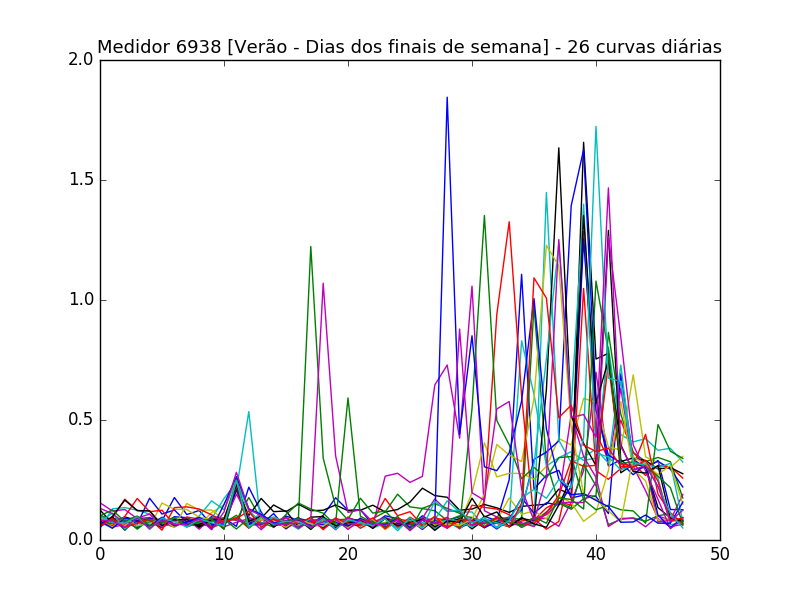
\includegraphics[width=.9\linewidth]{figuras/irish/raw_data_6938.png}
		\caption{Versão não normalizada.}
		\label{fig:6938_raw}
	\end{subfigure}%
	\begin{subfigure}{.5\textwidth}
		\centering
		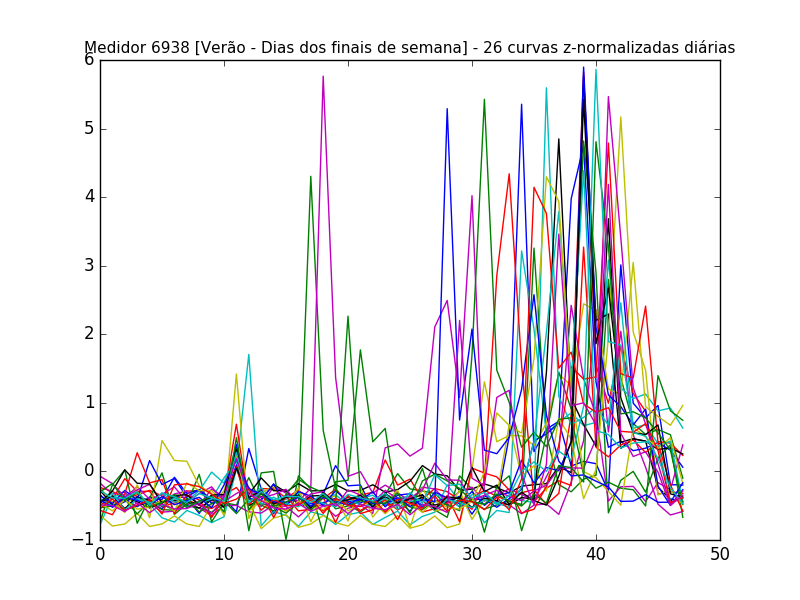
\includegraphics[width=.9\linewidth]{figuras/irish/Z_norm_6938.png}
		\caption{Versão z-normalizada.}
		\label{fig:6938_Z}
	\end{subfigure}
	\caption{Curvas de consumo diárias medidas pelo medidor 6938 no verão de 2010 contendo somente curvas de dias dos finais de semana (sábado e domingo).}
	\label{fig:Z_norm}
\end{figure}

%\begin{figure}[h!]
%	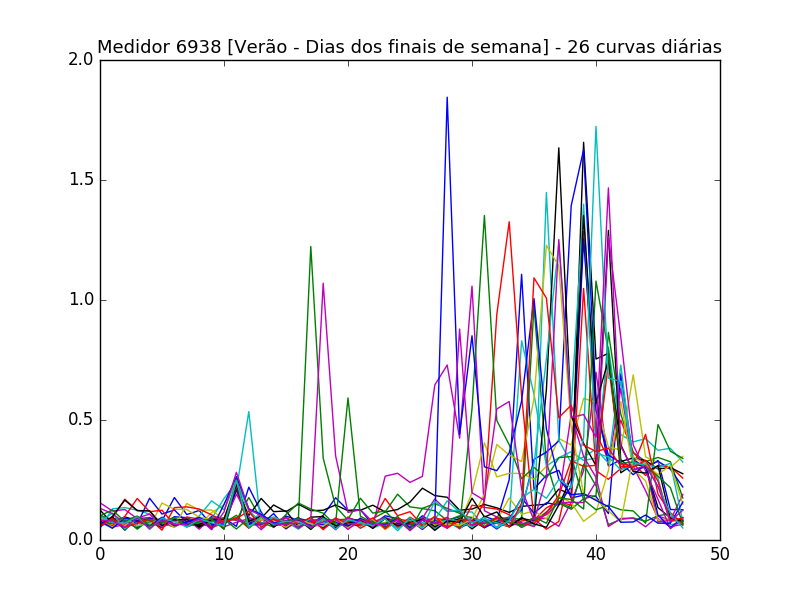
\includegraphics[width=\linewidth]{figuras/irish/raw_data_6938.png}
%	\caption{Curvas de consumo diárias medidas pelo medidor 6938 no verão de 2010 contendo somente curvas de dias dos finais de semana (sábado e domingo).}
%	\label{fig:6938_raw}
%\end{figure}

%\begin{figure}[h!]
%	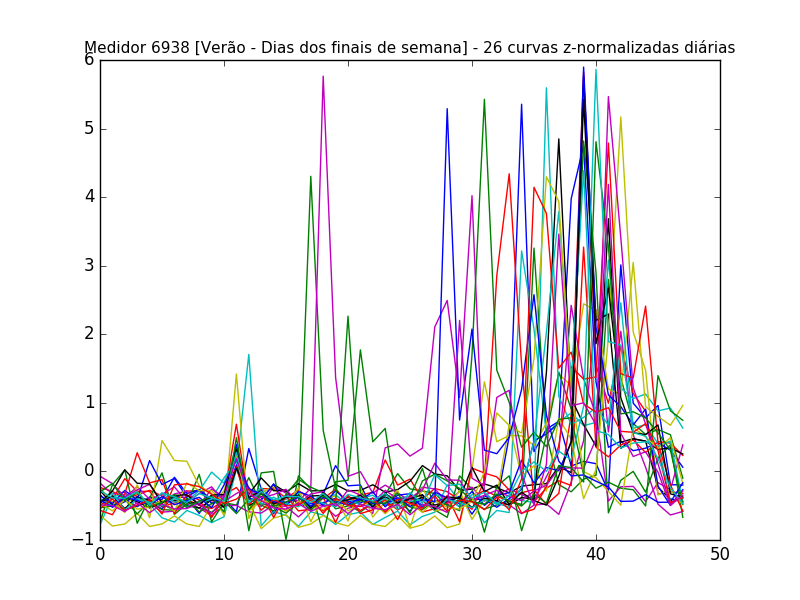
\includegraphics[width=\linewidth]{figuras/irish/Z_norm_6938.png}
%	\caption{Versão z-normalizada das curvas da figura ~\ref{fig:6938_raw}}
%	\label{fig:6938_Z}
%\end{figure}

Após a criação desses sub-conjuntos de dados, foi escolhida uma curva diária de cada medidor para cada sub-conjunto, de forma que tal curva seja o mais representativa possível do medidor naquele subconjunto. Diferentemente de ~\parencite{Flath2012}, onde obteve-se o centróide para cada medidor em cada subconjunto e em seguida os dados foram normalizados pela normalização max \hl{TODO: citar normalizacao max}, neste trabalho,  primeiramente, todas as curvas diárias de cada medidor foram z-normalizadas, conforme descrito na seção ~\ref{sec:norm_Z}. Após esta etapa de normalização, as distâncias cid-euclidiana entre as curvas de cada medidor, em cada um dos $6$ sub-conjuntos foram calculadas, de forma que o medóide de cada medidor foi obtido e escolhido como o mais representativo de  cada medidor em cada subconjunto de dados. O medóide encontrado para as curvas do medidor 6938 representados na figura ~\ref{fig:6938_Z} pode ser visto na figura ~\ref{fig:6938_medoid},

\begin{figure}[h!]
	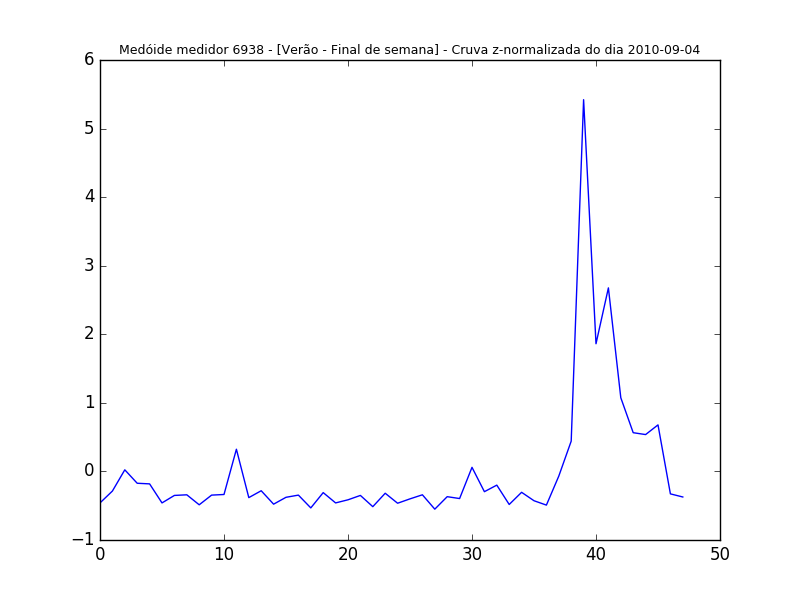
\includegraphics[width=\linewidth]{figuras/irish/medoid_6938.png}
	\caption{Medóide encontrado para as curvas da figura ~\ref{fig:6938_Z}}
	\label{fig:6938_medoid}
\end{figure}


Escolheu-se esta estratégia pelo fato todos os estudos terem sido feitos com a normalização Z e pela reconhecimento de sua superioridade em relação às demais normalizações no contexto de séries temporais. Já a preferência do medóide em detrimento do centróide, se deu pelo fato de esse ser menos sensível a \emph{outliers} do que este, de forma que se, dentro de determinada estação do ano, em um dia de semana por exemplo, houver algum consumo de energia atípico, como ocorre em feriados, tal efeito será desconsiderado, ou pelo menos atenuado, caso se escolha o medóide como curva mais representativa. No entanto, o mesmo não poderia ser dito caso fosse escolhido o centróide como a curva mais representativa.

Após esta etapa da escolha da curva do medidor mais representativo de cada sub-conjunto fez-se necessário o descarte de mais alguns medidores com dados anômalos. Primeiro todos os medidores que apresentavam valores constantes foram descartados, pois estes formam um grupo pequeno que possui um perfil muito bem definido e significativamente diferente dos perfis de consumo dos demais medidores. Caso os medidores com valores de medição constante não fossem descartados, isso faria com que a tarefa de agrupamento indicasse a presença de apenas $2$ grupos muito bem definidos, sendo um dos grupos formado por um pequeno número de medidores com valores constantes e o outro grupo com todos os outros medidores que possuem variações em sua medição. O número de medidores descartados em cada subconjunto nesta etapa se encontra detalhado na coluna 'Constantes descartados' da tabela ~\ref{tbl:sumario_descarte}.

Após o descarte dos medidores com medidas constantes foi calculada a matriz de dissimilaridade para cada um dos 6 subconjuntos, utilizando-se a métrica cid-euclidiana. Uma vez obtida a matriz de dissimilaridade para cada subconjunto, foi encontrado o medóide de cada subconjunto. Uma vez definido o medóide, que é a curva diária mais representativa de todos os medidores daquele subconjunto, calculou-se a média e o desvio padrão das dissimilaridades entre cada instância e o medóide. A partir daí, verificou-se que existem alguns medidores que se encontram significativamente afastados do medóide, de maneira que estes também foram descartados. Foi calculada a dissimilaridade média e o desvio padrão das instâncias até o medóide, e os medidores que apresentavam uma dissimlaridade cid-euclidiana em relação ao medóide maior que a média mais duas vezes o desvio padrão foram descartados. O número de medidores descartados nesta segundo etapa para cada subconjunto se encontra detalhado na coluna '\emph{outliers} descartados' da tabela ~\ref{tbl:sumario_descarte}. \hl{TODO: Ver com Cristiano se deve-se utilizar a distancia Mahalanobis aqui. Acho que nao}

Finalmente, na última etapa do pré-processamento, com a finalidade de manter-se a coerência entre os subconjuntos, ou seja, de que todos os subconjuntos contenham os dados de medição dos mesmos medidores, alguns medidores ainda foram descartados. O número de medidores descartados nesta etapa final em cada subconjunto e em cada uma das etapas de pré-processamento anteriores se encontra sumarizado na coluna 'Descartados na etapa final' da tabela ~\ref{tbl:sumario_descarte}. Ao final da etapa de pré-processamento todos os subconjuntos continham as medidas dos mesmos $4996$ medidores do conjunto inicial, ou seja, na etapa de pré-processamento foram descartados $1439$ medidores do conjunto original da Irlanda o que representa, aproximadamente, $22\%$ do número de medidores inicial.

\begin{center}
	\begin{table}			
		\caption{Tabela que sumariza os números de medidores descartados em cada uma das etapas de pré-processamento em cada um dos subconjuntos. Ao final, todos os subconjuntos contêm os mesmos $4996$ medidores. } 
	\resizebox{\columnwidth}{!}{%
	\begin{tabular}{llllll}
		\toprule
		Id &          Estação do Ano &              Dia de semana? & Constantes descartados & \emph{outliers} descartados & Descartados na etapa final\\
		\midrule
		S\_weekend  &  Verão       &  Não &             71 & 281 &  256\\
		S\_weekday  &   Verão      &  Sim &               63 & 233 & 316  \\
		W\_weekend &  Inverno    &  Não &               52 & 203 & 253\\
		W\_weekday &  Inverno    &  Sim &            41 & 65 & 306\\
		T\_weekend  &  Transição &   Não &               89 & 291 & 228\\
		T\_weekday  &   Transição &  Sim &          81 & 260 & 271\\
		\bottomrule
	\end{tabular}
	}
		\end{table} \label{tbl:sumario_descarte}
\end{center}

\section{Agrupamento das curvas de carga}

Após a etapa de pré-processamento, faz-se necessária a definição do número de grupos de cada um dos $6$ subconjuntos, já que é possível, e se espera, que existam subconjuntos com um número de grupos diferentes. Para tal, iremos utilizar as estratégias definidas na seção ~\ref{sec:definicao_indice_interno}, no qual cada subconjunto será agrupado pelo algoritmo hierárquico com linkagem \emph{average}, e o dendrograma resultante será podado para valores iterativos de $k$, que é o número de grupos. O valor de $k$ que acarretar no melhor valor do índice de Calinski-Harabasz será o número de grupos daquele subconjunto. Como dito, a escolha do índice se baseia nos experimentos da seção ~\ref{sec:indice_iterativo}, pois em ~\parencite{Flath2012} foi utilizado o índice Davies-Bouldin.

O intervalo de número de grupos testado foi de $2$ grupos até $9$ grupos, pois este é um intervalo no qual faz sentido a divisão de perfis de carga para a criação de políticas de tarifas diferentes para cada grupo. Ou seja, é possível que um valor de $k$ maior do que o limite superior do intervalo possua um valor melhor para o índice Calinski-Harabasz, no entanto, para a aplicação em questão, ele não faz sentido. O número de grupos escolhido para cada subconjunto se encontram na tabela ~\ref{tbl:valores_otimos_k} e os valores iterativos detalhados na tabela ~\ref{tbl:valores_iterativos_k}.

\begin{center}
			\begin{table}
				\caption{Tabela que mostra a variação do índice Calinski-Harabasz para valores iterativos do número de grupos. Os valores ótimos para cada subconjunto se encontram destacados. } 
%	\resizebox{\columnwidth}{!}{% 
		\begin{tabular}{llrrrrrrrr}
			\toprule
			{} &    subconjunto &    k=2 &     k=3 &      k=4 &     k=5 &     k=6 &     k=7 &     k=8 &     k=9 \\
			\midrule
			 &  S\_weekday &   7.31 &   47.14 &    28.17 &  \bfseries{799.96 } &  647.15 &  551.76 &  478.84 &  433.44 \\
			 &  S\_weekend &  83.77 &   60.10 &  \bfseries{1216.29} &  913.81 &  753.17 &  629.40 &  539.54 &  494.46 \\
			 &  T\_weekday &  51.96 &  172.64 &   128.53 &   96.47 &  101.20 &   84.51 &  \bfseries{469.90} &  411.93 \\
			 &  T\_weekend &  16.66 &   68.36 &    52.28 &  191.03 &  \bfseries{858.14} &  715.85 &  614.17 &  537.50 \\
			 &  W\_weekday &   7.74 &   44.12 &    30.20 &   24.00 &   19.21 &   15.86 &  \bfseries{549.97} &  481.31 \\
			 &  W\_weekend &   1.44 &   30.93 &    \bfseries{44.24} &   35.17 &   27.92 &   31.70 &   27.12 &   23.68 \\
			\bottomrule
		\end{tabular} 	
\end{table}\label{tbl:valores_iterativos_k}
%	}

\end{center}

\begin{center}
	\begin{table}
		\caption{Tabela que mostra os valores ótimos de cada subconjunto segundo o índice de Calinski-Harabasz.} 		
%	\resizebox{\columnwidth}{!}{%
\begin{tabular}{lll}
 	\toprule
 	{} &    subconjunto & $k\_\{opt\}$ \\
 	\midrule
 	 &  S\_weekday &       5 \\
 	 &  S\_weekend &       4 \\
 	 &  T\_weekday &       8 \\
 	 &  T\_weekend &       6 \\
 	 &  W\_weekday &       8 \\
 	 &  W\_weekend &       4 \\
 	\bottomrule
\end{tabular}	
	\end{table}\label{tbl:valores_otimos_k}
%	} 
\end{center} 	

Uma vez definido o número de grupos para cada subconjunto, agora para se encontrar a melhor partição realizaremos os procedimentos definidos na seção ~\ref{sec:indice_interno_k_fixo}. Nela chegou-se a conclusão que a melhor partição de um conjunto de dados de séries temporais é obtida ao se variar as estratégias de agrupamento para valores fixos de $k$, e a estratégia que apresentar os melhores valores do índice de silhouette será a partição escolhida. Por estratégia de agrupamento entende-se as variações de algoritmos de agrupamento e métrica de dissimilaridade. As estratégias testadas bem como os valores de silhouette para cada subconjunto podem ser vistos  na tabela ~\ref{tbl:valores_silhouette}.

\begin{center}
	\begin{table}
		\caption{Valores para o silhouette para diferentes estratégias em cada de cada subconjunto, onde HA representa a escolha do algoritmo hieráquico com linkagem \emph{average}.} 		
	\resizebox{\columnwidth}{!}{%
\begin{tabular}{lrrrrrrrrrrrrr}
	\toprule
	dataset & k-means,eucl & HA,DTW & HA,EDR & HA,chebyshev & HA,cid-DTW & HA,cid-EDR & HA,cid-chebyshev & HA,cid-eucl & HA,cort-DTW & HA,cort-EDR & HA,cort-chebyshev & HA,cort-eucl & HA,eucl \\
	\midrule
	S\_weekday &                0.06 &                     0.17 &                     0.17 &                           0.07 &                         0.19 &                         \bfseries{0.21} &                               0.09 &                                 0.07 &                          0.11 &                          0.17 &                                0.05 &                                  0.05 &                             0.05 \\
	S\_weekend &                0.06 &                     0.15 &                     0.25 &                           0.08 &                         0.20 &                         \bfseries{0.31} &                               0.08 &                                 0.13 &                          0.17 &                          0.24 &                                0.05 &                                  0.04 &                             0.06 \\
	T\_weekday &                0.06 &                     0.14 &                     \bfseries{0.15} &                           0.07 &                         0.11 &                         0.13 &                               0.04 &                                 0.04 &                          0.06 &                          0.12 &                                0.02 &                                  0.03 &                             0.05 \\
	T\_weekend &                0.06 &                     0.15 &                     0.21 &                           0.04 &                         0.20 &                         \bfseries{0.24} &                               0.05 &                                 0.10 &                          0.11 &                          0.17 &                                0.03 &                                  0.04 &                             0.06 \\
	W\_weekday &                0.05 &                     0.15 &                     0.15 &                           0.12 &                         \bfseries{0.22} &                         0.10 &                               0.13 &                                 0.05 &                          0.16 &                          0.14 &                                0.03 &                                  0.06 &                             0.10 \\
	W\_weekend &                0.05 &                     \bfseries{0.26} &                     0.23 &                           0.17 &                         0.16 &                         0.17 &                               0.20 &                                 0.15 &                          0.25 &                          0.21 &                                0.13 &                                  0.16 &                             0.15 \\
	\bottomrule
\end{tabular}
	}
	\end{table}\label{tbl:valores_silhouette}
\end{center} 

\begin{center}
	\begin{table}
		\caption{Tabela que mostra os resultados do agrupamento de cada subconjunto.} 		
		%	\resizebox{\columnwidth}{!}{%
		\begin{tabular}{lllll}
			\toprule
			subconjunto & $k\_\{opt\}$ & Algoritmo de agrupamento & Medida de dissimilaridade & Silhouette \\
			\midrule
			 S\_weekday &       5 & hierarchical-average & cid-EDR & 0.21 \\
			 S\_weekend &       4 & hierarchical-average & cid-EDR & 0.31\\
			 T\_weekday &       8 & hierarchical-average & EDR & 0.15 \\
			 T\_weekend &       6 & hierarchical-average & cid-EDR & 0.24 \\
			 W\_weekday &       8 & hierarchical-average & cid-DTW & 0.22 \\
			 W\_weekend &       4 & hierarchical-average & DTW & 0.25\\
			\bottomrule
		\end{tabular}	
	\end{table}\label{tbl:resultados_finais_agrupamento}
	%	} 
\end{center} 

Os medóides de cada grupo bem como o número de cargas em cada grupo podem ser vistos nas figuras a seguir.

\begin{figure}[h!]
	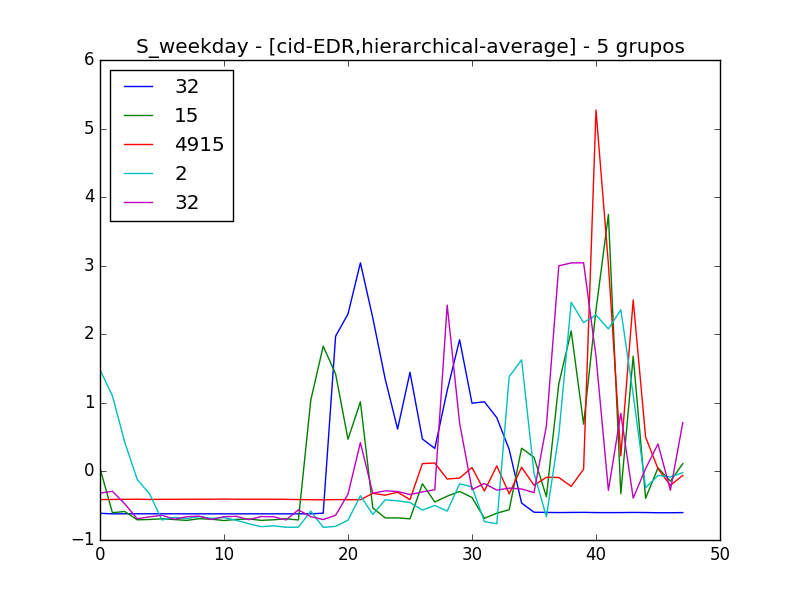
\includegraphics[width=\linewidth]{figuras/irish/2016-07-19_15:33:04.743952__irish_results/S_weekday_-_[cid-EDR,hierarchical-average]_-_5_grupos.png}
	\caption{Medóide encontrado para as curvas...}
	%\label{fig:6938medoid}
\end{figure}

\begin{figure}[h!]
	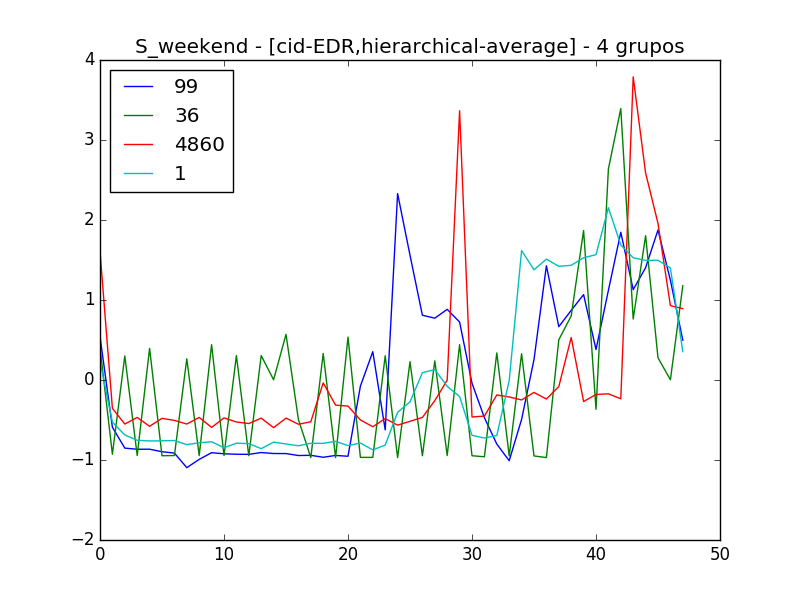
\includegraphics[width=\linewidth]{figuras/irish/2016-07-19_15:33:04.743952__irish_results/S_weekend_-_[cid-EDR,hierarchical-average]_-_4_grupos.png}
	\caption{Medóide encontrado para as curvas...}
	%\label{fig:6938medoid}
\end{figure}

\begin{figure}[h!]
	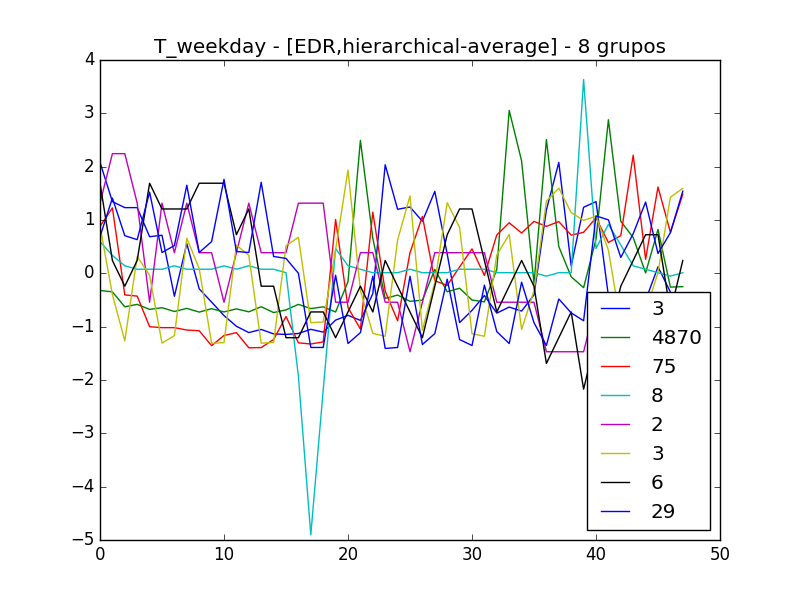
\includegraphics[width=\linewidth]{figuras/irish/2016-07-19_15:33:04.743952__irish_results/T_weekday_-_[EDR,hierarchical-average]_-_8_grupos.png}
	\caption{Medóide encontrado para as curvas...}
	%\label{fig:6938medoid}
\end{figure}

\begin{figure}[h!]
	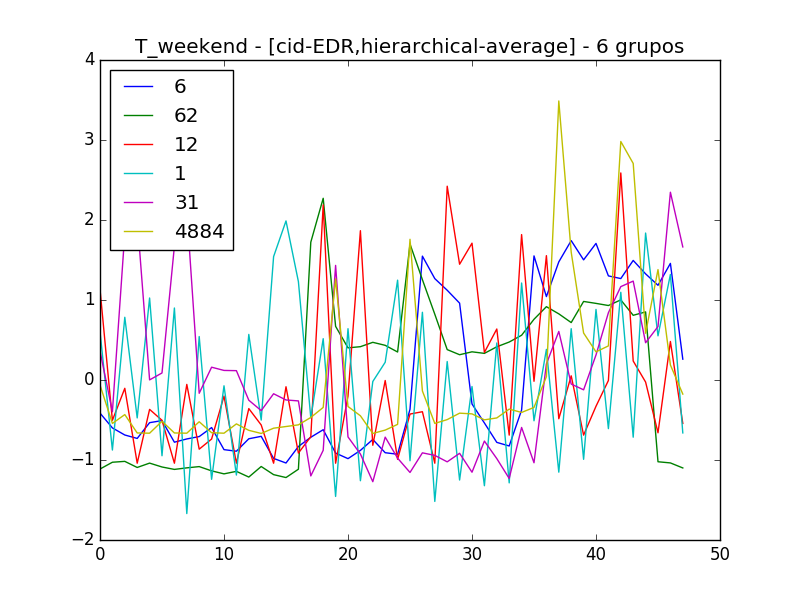
\includegraphics[width=\linewidth]{figuras/irish/2016-07-19_15:33:04.743952__irish_results/T_weekend_-_[cid-EDR,hierarchical-average]_-_6_grupos.png}
	\caption{Medóide encontrado para as curvas...}
	%\label{fig:6938medoid}
\end{figure}

\begin{figure}[h!]
	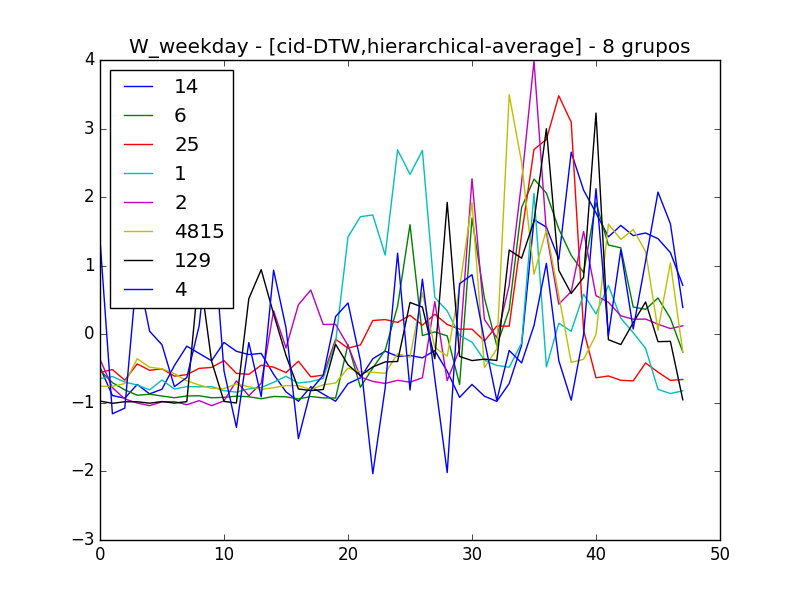
\includegraphics[width=\linewidth]{figuras/irish/2016-07-19_15:33:04.743952__irish_results/W_weekday_-_[cid-DTW,hierarchical-average]_-_8_grupos.png}
	\caption{Medóide encontrado para as curvas...}
	%\label{fig:6938medoid}
\end{figure}

\begin{figure}[h!]
	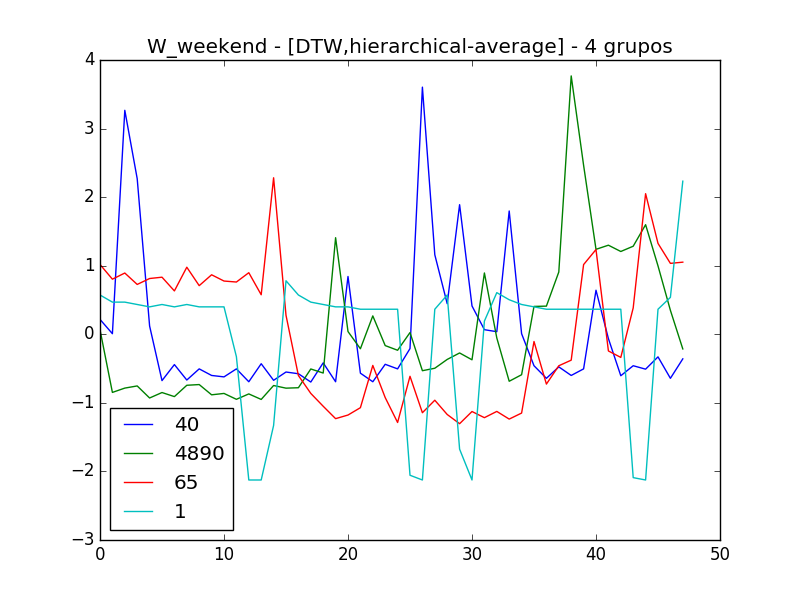
\includegraphics[width=\linewidth]{figuras/irish/2016-07-19_15:33:04.743952__irish_results/W_weekend_-_[DTW,hierarchical-average]_-_4_grupos.png}
	\caption{Medóide encontrado para as curvas...}
	%\label{fig:6938medoid}
\end{figure}

\section{Análise e discussão dos resultados}


